\documentclass[handout]{beamer}
%\usepackage[margin=1in]{geometry}
\usepackage{amsthm,amsmath,amsfonts,hyperref,graphicx,color,multicol}
\usepackage{enumitem,tikz}

%%%%%%%%%%
%Beamer Template Customization
%%%%%%%%%%
\setbeamertemplate{navigation symbols}{}
\setbeamertemplate{theorems}[ams style]
\setbeamertemplate{blocks}[rounded]

\definecolor{Blu}{RGB}{43,62,133} % UWEC Blue
\setbeamercolor{structure}{fg=Blu} % Titles

%Unnumbered footnotes:
\newcommand{\blfootnote}[1]{%
	\begingroup
	\renewcommand\thefootnote{}\footnote{#1}%
	\addtocounter{footnote}{-1}%
	\endgroup
}


%%%%%%%%%%
%Custom Commands
%%%%%%%%%%
\newcommand{\R}{\mathbb{R}}
\newcommand{\veca}{\vec{a}}
\newcommand{\vecb}{\vec{b}}
\newcommand{\vece}{\vec{e}}
\newcommand{\vecu}{\vec{u}}
\newcommand{\vecv}{\vec{v}}
\newcommand{\vecw}{\vec{w}}
\newcommand{\vecx}{\vec{x}}
\newcommand{\zerovector}{\vec{0}}

\newcommand{\ds}{\displaystyle}

\newcommand{\fn}{\insertframenumber}

\newcommand{\rank}{\operatorname{rank}}
\newcommand{\adj}{\operatorname{adj}}

\newcommand{\blank}[1]{\underline{\hspace*{#1}}}


%%%%%%%%%%
%Custom Theorem Environments
%%%%%%%%%%
\theoremstyle{definition}
\newtheorem{exercise}{Exercise}
\newtheorem{question}[exercise]{Question}
\newtheorem*{defn}{Definition}
\newtheorem*{exa}{Example}
\newtheorem*{disc}{Group Discussion}
\newtheorem*{nb}{Note}
\newtheorem*{recall}{Recall}
\renewcommand{\emph}[1]{{\color{blue}\texttt{#1}}}

\definecolor{Gold}{RGB}{237, 172, 26}
%Statement block
\newenvironment{statementblock}[1]{%
	\setbeamercolor{block body}{bg=Gold!20}
	\setbeamercolor{block title}{bg=Gold}
	\begin{block}{\textbf{#1.}}}{\end{block}}

\begin{document}
	\title{Math 324: Linear Algebra}
	\subtitle{2.5: Applications of Matrix Operations}
	\author{Mckenzie West}
	\date{Last Updated: \today}
\begin{frame}
\maketitle
\end{frame}

\begin{frame}{\insertframenumber}
	\begin{block}{\textbf{Last Time.}}
	\begin{itemize}[label=--]
		\item Theorem 2.15
		\item Elementary Matrices
		\item Row Equivalence
		\item Writing a Matrix as a Product of Elementary Matrices
		\item Elementary Matrices and Inverses
	\end{itemize}
	\end{block}
\begin{block}{\textbf{Today.}}
	\begin{itemize}[label=--]
		\item Stochastic Matrices
		\item Consumer Preference Models
		\item Cryptography-Encoding and Decoding using Matrices
		\item Leontief Input-Output Models
		\item Least Squares Approximation
	\end{itemize}
\end{block}
\end{frame}


\begin{frame}{\fn}
	\begin{defn}
		A \emph{stochastic matrix} is an $n\times n$ matrix $P$ where every entry is in the interval $[0,1]$ and the sum of the entries in each column is 1.
	\end{defn}

	\begin{nb}
		Stochastic matrices are used to describe probabilities of going from one state to the next, also called \emph{transition probabilities}.
	\end{nb}
\end{frame}

\begin{frame}{\fn}
	\begin{exercise}
		A population of 10,000 is grouped as follows: 5000 nonsmokers, 2500 smokers of one pack or less per day, and 2500 smokers of more than one pack per day.  During any month, there is a 5\% probability that a nonsmoker will begin smoking a pack or less per day, and a 2\% probability that a nonsmoker will begin smoking more than one pack a day.  For smokers who smoke a pack or less per day, there is a 10\% probability of quitting and a 10\% probability of increasing to more than a pack per day.  For smokers who smoke more than a pack per day, there is a 5\% probability of quitting and a 10\% probability of dropping to a pack or less per day.  How many will be in each group (a) in 1 month and (b) in 2 months?
		\footnote{Section 2.5 Exercise 7}
	\end{exercise}
\end{frame}
\begin{frame}{\fn}
\begin{exercise}
	An escape room designer places a person in a locked space with three compartments, as show in the figure below--the diamonds represent doors.  The person has been instructed to select a door at random whenever a bell is rung and to move through it into the next compartment. Note that the person is equally likely to go through any of the doors in their current room.
	\begin{center}
	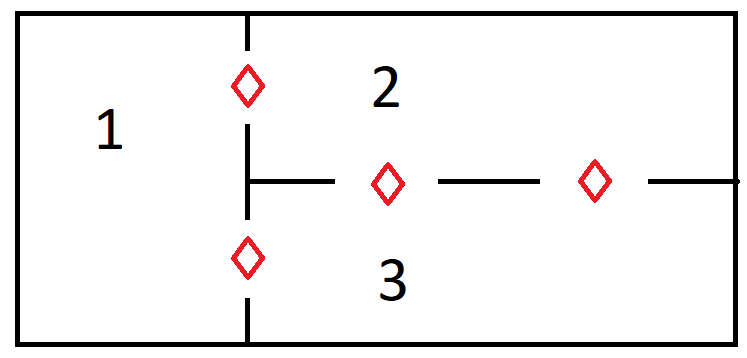
\includegraphics[width=2in]{images/markov1}
	\end{center}
	\begin{enumerate}[label=(\alph*)]
		\item Write down a stochastic matrix where the $(i,j)$ entry describes the probability that the person moves from room $j$ to room $i$.
	\end{enumerate}
\end{exercise}
\end{frame}
\begin{frame}{\fn}
\begin{block}{\textbf{Exercise 2.} (Continued)}
	\begin{enumerate}[label=(\alph*)]
		\item[(b)] If the person starts in room 1, what is the probability that the person will be in room 2 after the bell has rung twice? three times?\pause
		\item[(c)] It turns out that ``escape room designer'' was never going to let the person leave but instead will just keep ringing the bell into eternity.  In the long run, what proportion of time will the person spend in each room?
	\end{enumerate}
\end{block}
\end{frame}

%\begin{frame}{\fn}
%\begin{exercise}
%	The following information is proposed in by archaeologists. [D.H. Thomas, ``A Computer Simulation Model of Great Basin Shoshonean Subsistence and Settlement Patterns,'' in D.L. Clarke, ed., \textit{Models in Archaeology} (London: Methuen, 1972).]
%	
%	They studies the quality of pine nut crops from 1940 to 1947, and postulated that the probabilities of good crops could be modeled with stochastic matrices:\footnote{p246 of D. Poole, \textit{Linear Algebra: A Modern Introduction}, 4ed.}
%	\begin{itemize}[label=--]
%		\item good one year $\rightarrow$ the following year's crop would be good, fair, or poor with probability 0.08, 0.07, and 0.85, respectively;
%		\item fair one year $\rightarrow$ the following year's crop  would be good, fair, poor with probability 0.09, 0.11, and 0.80, respectively; 
%		\item poor one year $\rightarrow$ the following year's crop would be good, fair, or poor with probability 0.11, 0.05, and 0.84, respectively.
%	\end{itemize}
%	\begin{enumerate}[label=(\alph*)]
%		\item Write down a stochastic matrix representing these probabilities.
%	\end{enumerate}
%\end{exercise}
%%\end{frame}
%\begin{frame}{\fn}
%\begin{block}{\textbf{Exercise 3.} (Continued)}
%	\begin{enumerate}[label=(\alph*)]
%		\item[(b)] If the pine nut crop was good in 1940, find the probabilities of getting good crops in years 1941 thru 1945.
%		\item[(c)] In the long run, what proportion of crops will be good, medium poor?
%	\end{enumerate}
%\end{block}
%\end{frame}

\begin{frame}[fragile]{\fn}
	An $n\times n$ matrix can be used to encode a message by associating each letter with a number:
		\[A=1, B=2, C=3,\dots,Z=26\]
	with $0$ representing a space.
	\begin{exa}
		The message \texttt{HELLO WORLD} could be written as:  
			\[\begin{array}{ccccccccccc}
				H&E&L&L&O& &W&O&R&L&D\\
				8&5&12&12&15&0&23&15&18&12&4
			\end{array}\]
		If $n=4$, we write the message using
			\[\begin{bmatrix}8&5&12&12\end{bmatrix}\begin{bmatrix}15&0&23&15\end{bmatrix}
			\begin{bmatrix}18&12&4&0\end{bmatrix}\]
		To encode the message, we pick a random $4\times 4 $ invertible matrix (that we must remember or we won't be able to decode), and multiply it on the left by each of the $1\times 4$ row vectors.
	\end{exa}
\end{frame}
\begin{frame}{\fn}
\begin{exa}
	Continuing, let 
	\[A=\begin{bmatrix}
	3 & 4 & -3 & 2 \\
	4 & -2 & 5 & 4 \\
	5 & -4 & 3 & -3 \\
	1 & -1 & -2 & 1
	\end{bmatrix}\]
	Each encoded string is:\[\begin{array}{rcl}
	\begin{bmatrix}8&5&12&12\end{bmatrix}A&=&\begin{bmatrix}116&-38&13&12\end{bmatrix}\\
	\begin{bmatrix}15&0&23&15\end{bmatrix}A&=&\begin{bmatrix}175&-47&-6&-24\end{bmatrix}\\
	\begin{bmatrix}18&12&4&0\end{bmatrix}A&=&\begin{bmatrix}122&32&18&72\end{bmatrix}
	\end{array}\]
	What we would pass to our friend (who knows what $A$ is as well):
	\[116, -38, 13, 12, 175, -47, -6, -24, 122, 32, 18, 72\]
\end{exa}
\end{frame}
\begin{frame}{\fn}
	\begin{exercise}
		Suppose we're given $A=\begin{bmatrix}1&2\\3&5\end{bmatrix}$ and a message that was encoded using $A$:
	\[11, 21, 64, 112, 25, 50, 29, 53, 23, 46, 40, 75, 55, 92\]
	What was the original message?\footnote{Section 2.5 Exercise 15}
	\end{exercise}
\end{frame}
%\begin{frame}{\fn}
%\begin{exercise}\begin{enumerate}[label=(\alph*)]
%		\item 
%		Write a 10-25 character (including spaces) message to the table to your left (when looking at the TV).  
%	
%	\item Encode the message using an invertible $3\times 3$ matrix of your choosing.
%	
%	\item Pass the encoded message to the table to your left along with the matrix you used to encode the message.
%	
%	\item Then decode the message that was passed to your table. (You may return to this step if it looks like the table to your right is a few slides behind your pace.)
%	\end{enumerate}
%\end{exercise}
%\end{frame}
%\begin{frame}{\fn}
%\begin{exercise}
%	The following cryptogram was encoded with a $2\times 2$ matrix,
%	\[8, 21, -15, -10, -13, 5, 10, 5, 25, 5, 19, -1,6,20,40,-18,-18,1,16\]
%	The last word of the message is \underline{\hspace*{.1in}}RON.  What is the message?
%	\footnote{Section 2.5 Exercise 19}
%\end{exercise}
%\end{frame}
%\begin{frame}{\fn}
%\begin{exercise}\footnote{Section 2.5 Exercise 22}
%	You intercepted the following encoded message:
%	\[45, -35, 38, -30, 18, -18, 35, -30, 81, -60, 42, -28, 75,\]\[-55, 2,-3,22, -21,15,-10\]
%	
%	Let the inverse of the encoding matrix be:
%	\[A^{-1}=\begin{bmatrix}w&x\\y&z\end{bmatrix}\]
%	\begin{enumerate}[label=(\alph*)]
%		\item You know that $\begin{bmatrix}45&-36\end{bmatrix}A^{-1}=\begin{bmatrix}10&5\end{bmatrix}$ and  $\begin{bmatrix}38&-30\end{bmatrix}A^{-1}=\begin{bmatrix}8&14\end{bmatrix}$.  Write and solve two systems of equations to find $w,x,y$ and $z$.
%		\item Decode the message.
%	\end{enumerate}
%\end{exercise}
%\end{frame}

\begin{frame}{\fn}
	\begin{block}{\textbf{Brain Break.}}
		What was a “total first year move” you made when you began college?
		\begin{center}
			
\includegraphics[width=2in]{images/first_year}
		\end{center}
	\end{block}
\end{frame}


\begin{frame}{\fn}
	\begin{center}
		{\large\usebeamercolor[fg]{title}\textbf{Leontief Input-Output Models}}
		
		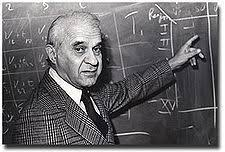
\includegraphics[width=1.5in]{images/leontief}
		
		{\footnotesize Image from: \href{https://www.goodreads.com/author/show/181430.Wassily_Leontief}{goodreads.com}}
	\end{center}
	Wassily Leontief, a Russian-American economist, won the 1973 Nobel prize in Economics for his work using the models he discovered.
\end{frame}

\begin{frame}{\fn}
	\begin{block}{\textbf{Idea.}}
		In an economic system, one company may use the outputs of another to produce its goods.  Example 7 in the book explains how Electricity, Water, and Coal power may need to supply one another in order to provide power to the public.
	\end{block}
	\begin{defn}
		A \emph{closed} system is one where all products are sold only to industries in the system.
		
		An \emph{open} system is one where some outputs are sold to non-producing industries outside the system.
	\end{defn}
\end{frame}

\begin{frame}{\fn}
	\begin{defn}
		Let $d_{ij}$ be the amount of output the $j$th industry needs from the $i$th industry to produce one unit of output per year.  The matrix formed by these values is called the \emph{input-output matrix}:
		\[D=\begin{bmatrix}d_{11}&d_{12}&\cdots&d_{1n}\\
		d_{21}&d_{22}&\cdots&d_{2n}\\
		\vdots&\vdots&&\vdots\\
		d_{n1}&d_{n2}&\cdots&d_{nn}\end{bmatrix}.\]
		
		That is rows correspond to input, columns correspond to output.
	\end{defn}
\end{frame}
\begin{frame}{\fn}
	\begin{exercise}\label{IO_one}
		A system composed of two industries, coal and steel, has the following input requirements:
		\begin{itemize}[label=--]
			\item to produce \$1.00 worth of output, the coal industry requires \$0.10 of its own product and \$0.80 of steel;
			\item to produce \$1.00 worth of output, the steel industry requires \$0.10 of its own product and \$0.20 of coal.
		\end{itemize}
		Find $D$, the input-output matrix for this system.
		\blfootnote{Section 2.5, Exercise 23}
	\end{exercise}
\end{frame}
\begin{frame}{\fn}
\begin{defn}
	If $X=\begin{bmatrix}x_1\\x_2\\\vdots\\x_n\end{bmatrix}$, the \emph{output matrix}, lists the total amounts produced by each industry, then 
	\[X=DX+E\]
	where $E$, the \emph{external demand matrix}, is the amount of product from each industry that is sold to the external industries.
\end{defn}
\begin{exercise}
	If you're given $D$ and $E$, how would you solve for $X$?
\end{exercise}
\end{frame}
\begin{frame}{\fn}
\begin{block}{\textbf{Exercise \ref{IO_one}.} (Continued)}
	For the coal and steel industries established in slide 13, assume the external demand matrix is $E=\begin{bmatrix}10000\\20000\end{bmatrix}$.
	\begin{enumerate}[label=(\alph*)]
		\item What do the 10,000 and 20,000 represent in the external demand matrix?
		\item Solve for the output matrix $X$ in the equation $X=DX+E$. *Be careful here about factoring.
	\end{enumerate}
\end{block}\pause
\begin{nb}
	One of the most incredible mathematical discoveries related to this work is the fact that $I-D$ is \textit{always} going to be invertible, given standard industry conditions.
\end{nb}
\end{frame}
\begin{frame}{\fn}
\begin{exercise}\blfootnote{Chapter 2 Review Exercise 72}
	An industrial system with three industries--chocolate, milk, and cookies--has the following input-output matrix $D$ and external demand matrix $E$:
	\[D=\begin{bmatrix}0.1&0.3&0.2\\0.0&0.2&0.3\\0.4&0.1&0.1\end{bmatrix}\textup{ and }E=\begin{bmatrix}3000\\3500\\8500\end{bmatrix}\]
	\begin{enumerate}[label=(\alph*)]
		\item Interpret each of the entries in the first column in terms of each of the industries.
		\item Interpret each of the entries in the second row in terms of each of the industries.
		\item Solve for the output matrix $X$ in the equation $X=DX+E$.
	\end{enumerate}
\end{exercise}
\end{frame}\begin{frame}{\fn}
\begin{defn}
	For a set of points $(x_1,y_1),\ (x_2,y_2),\dots,\ (x_n,y_n)$, the \emph{least squares regression line} is given by the linear function $f(x)=a_0+a_1x$ that minimizes the sum of squared error:
	\[[y_1-f(x_1)]^2+[y_2-f(x_2)]^2+\cdots+[y_n-f(x_n)]^2\]
\end{defn}
\end{frame}
\begin{frame}{\fn}
\begin{block}{\textbf{Finding the least squares regression line.}}
	\begin{itemize}[label=--]
		\item For the least squares approximation, we want 
		\[a+bx_1\approx y_1,a+bx_2\approx y_2,\dots,a+bx_n\approx y_n\]
		\item Let $X=\begin{bmatrix}
		1&x_1\\1&x_2\\\vdots&\vdots\\1&x_n
		\end{bmatrix}$, $Y=\begin{bmatrix}y_1\\y_2\\\vdots\\y_n\end{bmatrix}$, and $A=\begin{bmatrix}a\\b\end{bmatrix}$.
		We then condense all of the equations from above via:
		$XA\approx Y.$
		\item In fact, $A=(X^TX)^{-1}X^TY$.
		\item The individual errors for each $Y$ value are given by $E=Y-XA$.  The sum of square error is: $E^TE$.
	\end{itemize}
\end{block}
\end{frame}
\begin{frame}{\fn}
\begin{exercise}
	Find the least squares regression line for the data:
	\[(-5,1),(1,3),(2,3),(2,5).\]
	What is the sum of squared error?
\end{exercise}
\end{frame}
\begin{frame}{\fn}
\begin{exercise}
	The table shows the average salaries $y$ (in millions of dollars) or Major League Baseball players on opening day of baseball season from 2005 through 2010. (Source: Major League Baseball)\blfootnote{Chapter 2 Review Exercise 79}
	\begin{center}
		\begin{tabular}{r|cccccc}
			\hline
			Year & 2005&2006&2007 & 2008 & 2009 & 2010\\
			Salary, $y$ & 2.6&2.9 & 2.9&3.2&3.2&3.3\\
			\hline
		\end{tabular}
	\end{center}
	\begin{enumerate}[label=(\alph*)]
		\item Find the least squares regression line for the data. (I suggest translating the years like in Chapter 1).
		\item Use the linear model to create a table of estimated values for $y$ during the years 2005 to 2010.
		\item What is the sum of squared errors?
		\item What is the estimated salary for 2019?
		\item When, approximately, will the average salary be 6 million?
	\end{enumerate}
\end{exercise}
\end{frame}
\end{document}

 